\section{Introduction}

Over the past decade and a half, neutrino oscillation experiments have
been able to conclusively establish that neutrinos have mass
\cite{SNO2001,SNO2002,SuperK2002,kamland2003}. However, the nature of
that mass remains one of the most fundamental open questions in
particle physics. Is the neutrino unique among the Standard Model
fermions with a Majorana-type mass \cite{Majorana1937}, as is
predicted by most beyond the standard model (BSM) theories, or does it
have a Dirac-type mass like the rest of the fermions? A Majorana-type
mass would have far reaching implications, from explaining the
lightness of the neutrino and providing a bridge to higher energy
phenomena through the see-saw mechanism
\cite{GellMann1980,Yanagida1979} to being able to provide the required
lepton-number violation (LNV) and {\sf CP}-violation needed for
leptogenesis to explain the baryon asymmetry of the universe
\cite{Fukugita1986,Luty1992}. Conversely, a Dirac-type neutrino mass
could point to an underlying symmetry of the Universe.  Presently, the
most promising technique for answering these questions is the search
for Neutrinoless Double-Beta (0\nbb) decay \cite{Furry1939}. In this
decay, a nucleus undergoes a second order $\beta$-decay without
producing any neutrinos, $(Z,A)\rightarrow(Z+2,A)+2\beta^-$.  This is in comparison to two neutrino double beta (2{\nbb}) decay
\cite{GoeppertMayer1935}, the Standard Model allowed second order
\bmd-decay channel where lepton number is conserved by the
production of two anti-neutrinos, \mbox{$(Z,A)\rightarrow(Z,A+2)+2\beta+2\bar\nu_e$}.

%This is a detector paper so I don't think we need this detail.
%Recently, this search has generated a significant amount of
%experimental interest, with the largest on-going experiments searching
%for {0\nbb} decay of $^{76}$Ge \cite{GERDA2013}, $^{130}$Te
%\cite{CUORE2015,CUORE2016} and $^{136}$Xe
%\cite{EXO2014,KamLANDZen2013}. At present, 0{\nbb} decay has never
%been convincingly observed, but present limits indicate that the
%half-lives are longer than $10^{23}-10^{25}\,\mathrm{yr}$ in the
%isotopes studied. The standard mechanism of 0{\nbb} decay is
%parameterized by the \emph{effective Majorana mass}, defined as
%\mbox{$m_{\beta\beta}\equiv\left|\sum_i U^2_{ei}m_i\right|$}, where
%$U_{ei}$ are the elements of the PMNS matrix and $m_i$ are the
%neutrino masses. Current half-life limits translate to a limit on
%\mbox{$m_{\beta\beta}\lesssim 150-700\,\mathrm{meV}$}. The majority of
%the spread on this bound comes from theoretical uncertainty in the
%nuclear modeling (see \cite{Vogel2012} for a review). The next
%generation of 0{\nbb} decay experiments seek to be sensitive enough to
%detect or rule out 0{\nbb} decay down to \mbox{$m_{\beta\beta}\lesssim
%10$~meV}. This will require a detector to instrument roughly a ton
%of active isotope, maintain a good energy resolution, and achieve a
%near zero background in the region of interest (ROI) over the course
%of the experiment. % No citation needed I think, \cite{Cremonesi2013}.

Liquid scintillator-based detectors have
proven to be a competitive technology in this search\cite{KamLANDZen2013}. Their primary advantage is their ease of scalability to
larger instrumented masses, which involves dissolving larger amounts of
the isotope of interest into the liquid scintillator (LS). This
feature can allow for rapid scaling to 1~ton or more using the
detectors already in operation \cite{Biller2013}. In a large LS
detector, most backgrounds can be strongly suppressed through a
combination of filtration of the LS to remove internal contaminants,
self-shielding to minimize the effects of external contaminants, and
vetoes to reduce muon spallation backgrounds. The backgrounds relevant to
0{\nbb} decay which cannot be reduced through these means are the
2{\nbb} decay, electron scattering of $^8$B solar neutrinos and at more shallow depths long-lived spallation products especially $^{10}$C.
%(\tau=xx, Q=XX)$.

%\begin{figure}[ht]
%\centering
%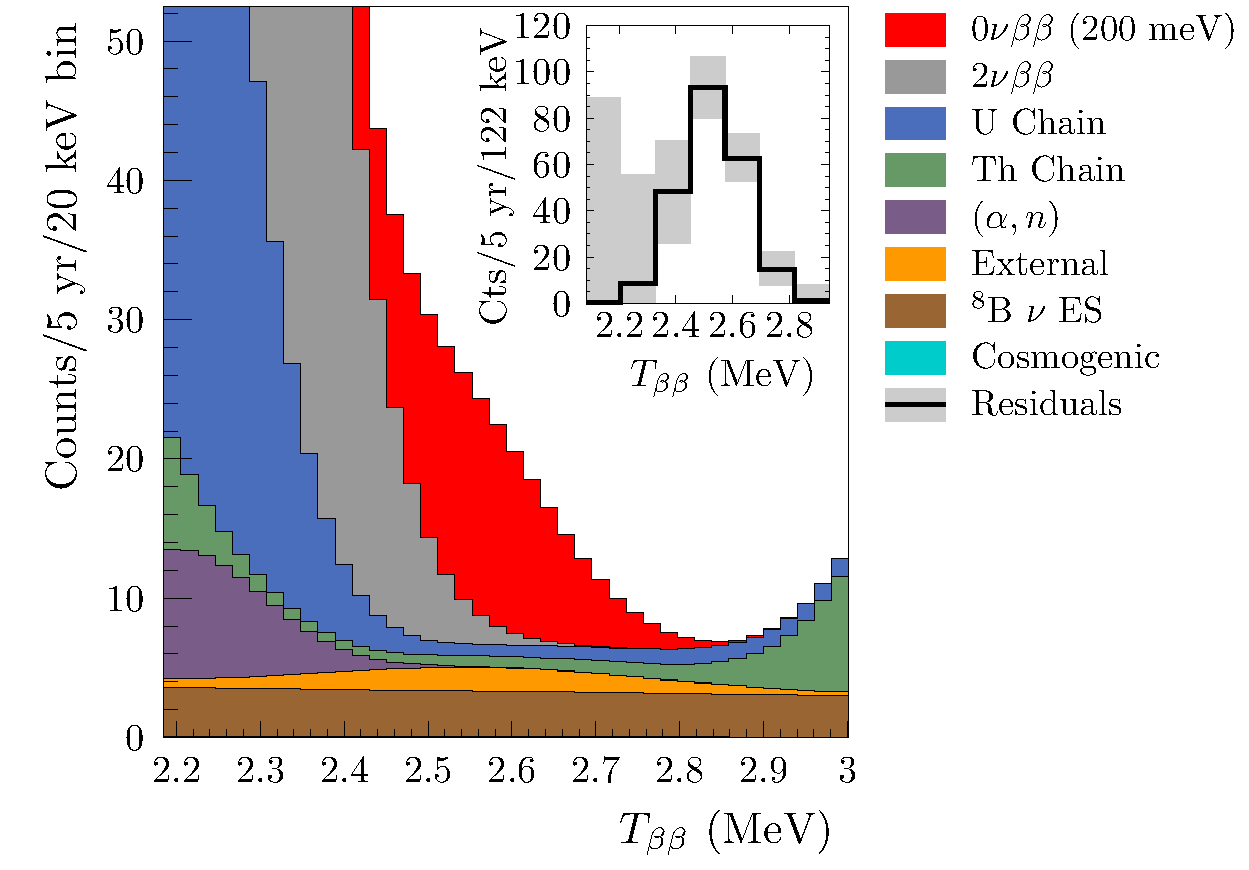
\includegraphics[width=0.49\columnwidth]{spectrum_plot_200_stack_nosums_nodata_inset_200mev.pdf}
%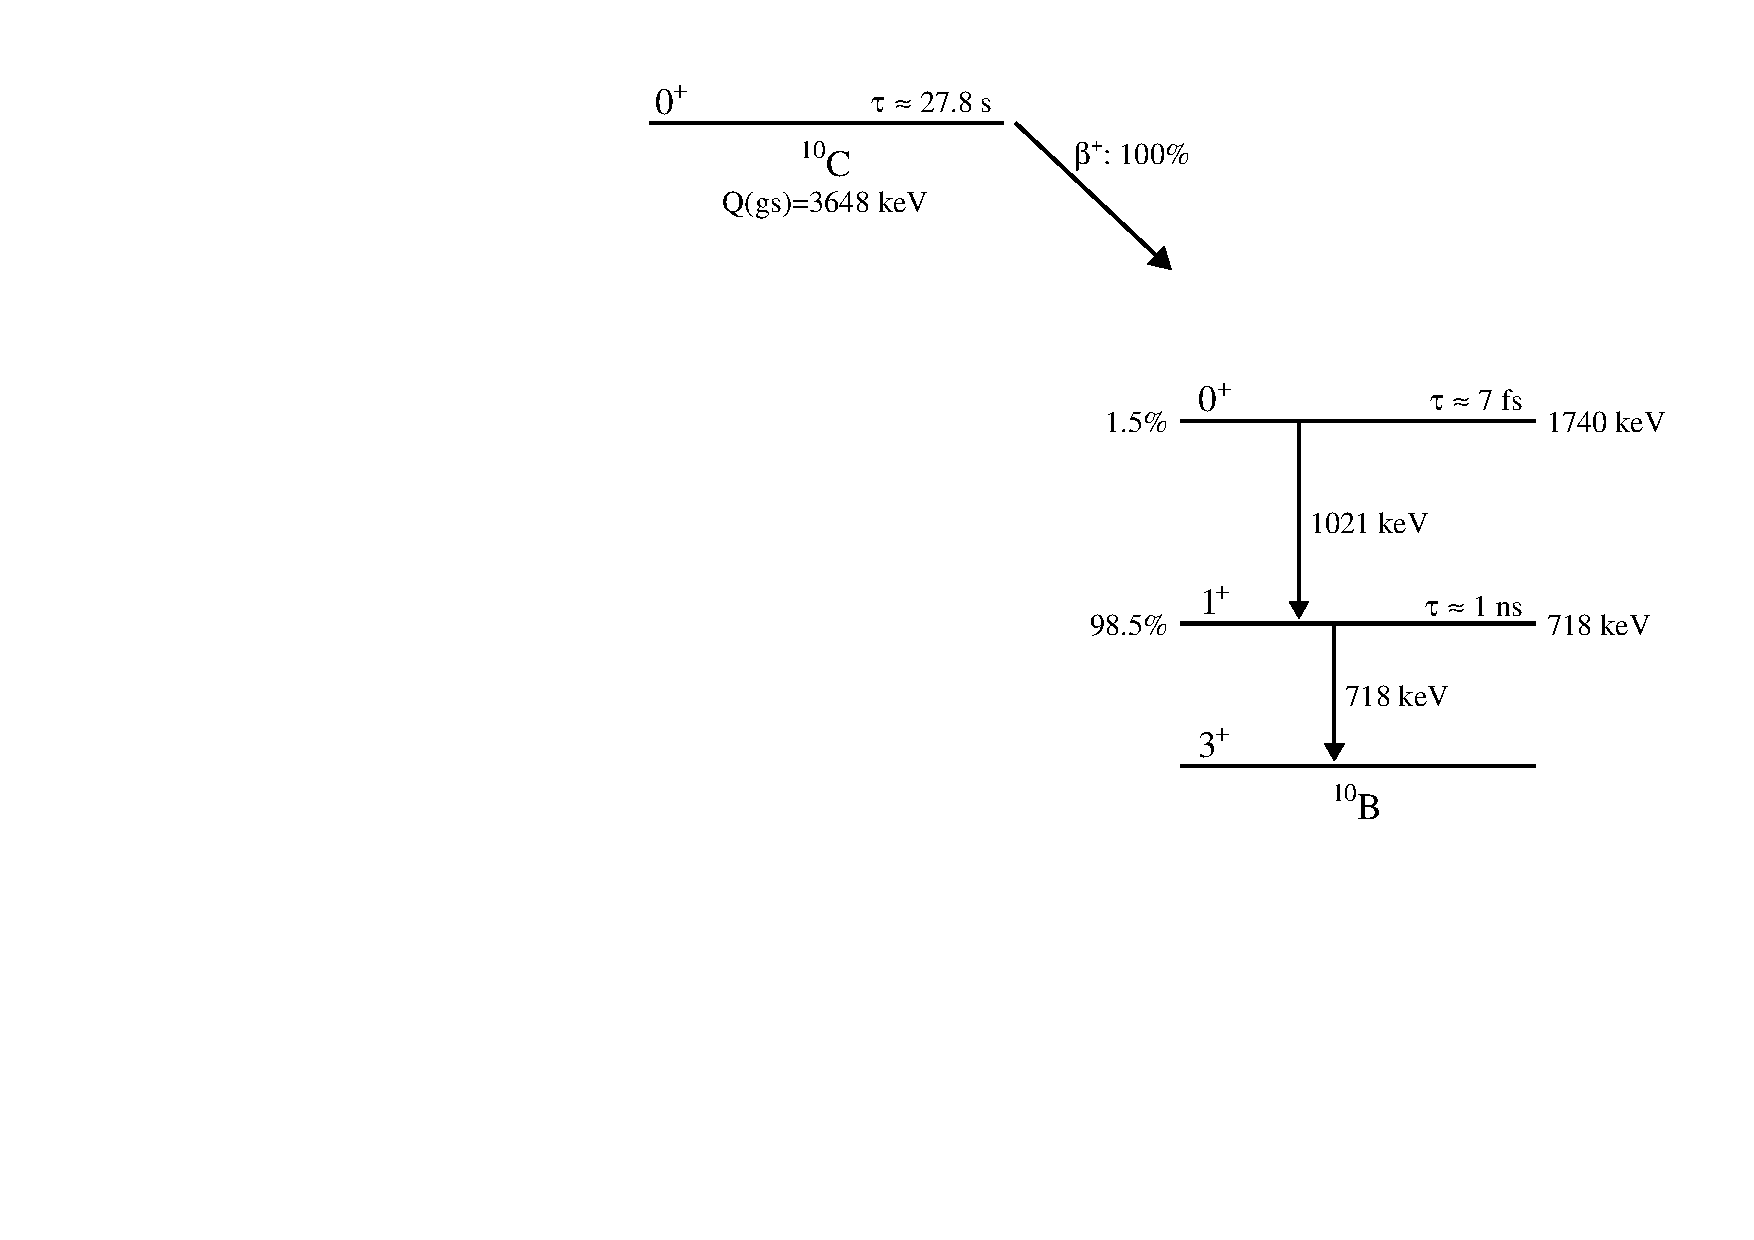
\includegraphics[width=0.49\columnwidth]{C10DecayScheme.pdf}
%\caption{ Plot taken from~\cite{SNOp_paper}}
%\label{fig:EdisAnd10C}
%\end{figure}


The 0{\nbb} signal and these backgrounds have distinctive energy spectra. Since 0{\nbb} decay produces no neutrinos, the full energy of the
decay is contained within the detector and a peak is observed around the decay $Q$-value. This defines a clear region of interest (ROI) around 
the $Q$-value. In 2{\nbb} decay, the neutrinos carry away some fraction of the decay energy leading to a broad spectrum from 0~MeV up to the 
decay $Q$-value. The interaction of \B~solar neutrinos through neutrino-electron elastic scatter (ES) produces produces a spectrum that rises 
at low energies, producing an effectively flat background in the ROI~\cite{SNOp-B8-bkg}. Finally, the \bpd-decay of \C~proceeds through a 
long lived excited state of \Bten. In a liquid scintillator detector, the full energy of the decay, positron kinetic energy, annihilation 
gammas, and de-excitation gammas, is detected. This results in a \bmd-decay spectrum offset from zero by $\sim$1.7~MeV, which corresponds
to the sum of energy of the gammas from the excited state and annihilation.

A detector with good energy resolution can statistically separate these backgrounds from the 0\nbb~ signal. Additional background rejection is possible with the inclusion of directional or topographical information. The two electrons emitted in 0\nbb~ and 2\nbb~ should reconstruct very differently than the single electron from ES or the positron and subsequent  gammas from the \C~decay. In previous work, we have shown that photo-detectors with timing resolution of $\sim$100~ps can be used to resolve the prompt Cherenkov photons from the slower scintillation signal and the resulting distributions can be fit for the position and direction of $\sim$MeV electrons\cite{Aberle2014}. 

In this paper, we examine in detail the time and topographical distributions of 0\nbb~ and these two key backgrounds. We propose a method 
using spherical harmonic decomposition to analyze the distribution of early photo-electrons (PE) and use this as a discriminant. 
In Section~\ref{sec:detector_description}, we describe the detector model we will use throughout this paper. Details on event kinematics and
PE timing for signal an backgrounds are given in Section~\ref{sec:kinematics_and_timing}
In Section~\ref{sec:topology_and_harmonics}, we introduce the spherical harmonic decomposition, and discuss the performance of this 
analysis in Section~\ref{sec:performance}.



%Since 0{\nbb} decay produces no neutrinos, the full energy of the
%decay is contained within the detector and the observed spectrum of
%this decay is a peak around the decay $Q$-value. Most of this energy
%is carried by the electrons which have typical kinetic energies of
%$\sim1-2\,\mathrm{MeV}$ each. Two neutrino double beta (2{\nbb}) decay
%\cite{GoeppertMayer1935} is the Standard Model allowed second order
%$\beta$-decay channel where lepton number is conserved by the
%production of two anti-neutrinos,
%\mbox{$(Z,A)\rightarrow(Z,A+2)+2\beta+2\bar\nu_e$}. Since the kinetic
%energy of the neutrinos is practically never detected, the energy
%spectrum measured from 2{\nbb} decay is broadened from 0~MeV up to the
%decay $Q$-value. Because it is intrinsic to the target isotope, the
%high energy tail of the 2{\nbb} spectrum forms an irreducible
%background to the 0{\nbb} signal. The only way to distinguish the two
%is through a shape analysis of the resulting decay spectrum. This
%requires a detector with a good energy resolution (see
%Fig.~\ref{fig:SNOp_bkgs}). Present LS-based detectors achieve typical
%energy resolutions of \mbox{$\sigma(E)\sim 5\%/\sqrt{E(\rm
%    MeV)}$}. The next generation of detectors will seek to improve
%upon this by increasing both the photo-covering of the detector and
%light yield of the LS. \JOcom{Eventually this will fold back in the
%  question of slowing down the scintillation signal and improving the
%  Cherenkov signal at the cost of decreasing the total light yield.}
  
%The spectrum of ES interactions of $^{8}$B solar neutrinos falls
%slowly over the range $2-3\,\mathrm{MeV}$, creating a nearly flat
%background across the ROI and reducing the sensitivity to 0{\nbb}. In
%this energy region, these interactions produce only a single
%$\sim$2.5~MeV electron, rather than two $\sim$1.2~MeV electrons as in
%0{\nbb}. In a LS, this difference in event topology manifests as two
%distinct distributions of Cherenkov photons, and thus creates a way to
%tag and remove these $^{8}$B solar neutrino events. As we have shown
%in previous works, photo-detectors with timing resolution of
%$\sim$100~ps can resolve the prompt Cherenkov photons from the slower
%scintillation signal \cite{Aberle2014}. The challenge is that for a
%given event, we expect $\sim$100 Cherenkov photons with which to
%reconstruct the event topology. \JOcom{It would be good to say
%something like: In a SNO/KamLAND sized detector, we expect $\sim$50
%  $^{8}$B events, so our rejection needs to be at least this good. But
%  perhaps we say that later?}








